\documentclass[12pt]{article}

\usepackage{graphics}
\usepackage{amsmath}
\usepackage{amsfonts}
\usepackage{amssymb}
\usepackage{blkarray}
\newcommand{\matindex}[1]{\mbox{\scriptsize#1}}
\usepackage[table]{xcolor}
\newcommand\scalemath[2]{\scalebox{#1}{\mbox{\ensuremath{\displaystyle #2}}}}



%\usepackage[active]{srcltx} % SRC Specials for DVI Searching

% Over-full v-boxes on even pages are due to the \v{c} in author's name
\vfuzz2pt % Don't report over-full v-boxes if over-edge is small

% THEOREM Environments ---------------------------------------------------

 \newtheorem{thm}{Theorem}[section]
 \newtheorem{cor}[thm]{Corollary}
 \newtheorem{lem}[thm]{Lemma}
 \newtheorem{prop}[thm]{Proposition}
 %\theoremstyle{definition}
 \newtheorem{defn}[thm]{Definition}
 %\theoremstyle{remark}
 \newtheorem{rem}[thm]{Remark}
 \numberwithin{equation}{section}
% MATH -------------------------------------------------------------------
 \DeclareMathOperator{\RE}{Re}
 \DeclareMathOperator{\IM}{Im}
 \DeclareMathOperator{\ess}{ess}
 \newcommand{\eps}{\varepsilon}
 \newcommand{\To}{\longrightarrow}
 \newcommand{\h}{\mathcal{H}}
 \newcommand{\s}{\mathcal{S}}
 \newcommand{\A}{\mathcal{A}}
 \newcommand{\J}{\mathcal{J}}
 \newcommand{\M}{\mathcal{M}}
 \newcommand{\W}{\mathcal{W}}
 \newcommand{\X}{\mathcal{X}}
 \newcommand{\BOP}{\mathbf{B}}
 \newcommand{\BH}{\mathbf{B}(\mathcal{H})}
 \newcommand{\KH}{\mathcal{K}(\mathcal{H})}
 \newcommand{\Real}{\mathbb{R}}
 \newcommand{\Complex}{\mathbb{C}}
 \newcommand{\Field}{\mathbb{F}}
 \newcommand{\RPlus}{\Real^{+}}
 \newcommand{\Polar}{\mathcal{P}_{\s}}
 \newcommand{\Poly}{\mathcal{P}(E)}
 \newcommand{\EssD}{\mathcal{D}}
 \newcommand{\Lom}{\mathcal{L}}
 \newcommand{\States}{\mathcal{T}}
 \newcommand{\abs}[1]{\left\vert#1\right\vert}
 \newcommand{\set}[1]{\left\{#1\right\}}
 \newcommand{\seq}[1]{\left<#1\right>}
 \newcommand{\norm}[1]{\left\Vert#1\right\Vert}
 \newcommand{\essnorm}[1]{\norm{#1}_{\ess}}
\usepackage{graphicx}
\usepackage{amsmath}
\usepackage{amsfonts}
\usepackage{amssymb}
%TCIDATA{OutputFilter=latex2.dll}
%TCIDATA{CSTFile=LaTeX article (bright).cst}
%TCIDATA{Created=Fri Nov 02 10:44:42 2001}
%TCIDATA{LastRevised=Mon Dec 10 11:56:49 2001}
%TCIDATA{<META NAME="GraphicsSave" CONTENT="32">}
%TCIDATA{<META NAME="DocumentShell" CONTENT="General\Blank Document">}
%TCIDATA{Language=American English}
\newtheorem{theorem}{Theorem}
\newtheorem{acknowledgment}[theorem]{Acknowledgment}
\newtheorem{algorithm}[theorem]{Algorithm}
\newtheorem{axiom}[theorem]{Axiom}
\newtheorem{case}[theorem]{Case}
\newtheorem{claim}[theorem]{Claim}
\newtheorem{conclusion}[theorem]{Conclusion}
\newtheorem{condition}[theorem]{Condition}
\newtheorem{conjecture}[theorem]{Conjecture}
\newtheorem{corollary}[theorem]{Corollary}
\newtheorem{criterion}[theorem]{Criterion}
\newtheorem{definition}[theorem]{Definition}
\newtheorem{example}[theorem]{Example}
\newtheorem{exercise}[theorem]{Exercise}
\newtheorem{lemma}[theorem]{Lemma}
\newtheorem{notation}[theorem]{Notation}
\newtheorem{problem}[theorem]{Problem}
\newtheorem{proposition}[theorem]{Proposition}
\newtheorem{remark}[theorem]{Remark}
\newtheorem{solution}[theorem]{Solution}
\newtheorem{summary}[theorem]{Summary}
\newenvironment{proof}[1][Proof]{\textbf{#1.} }{\ \rule{0.5em}{0.5em}}
\renewcommand\refname{}
\renewcommand\thefootnote{}
\textheight=9in \topmargin=-0.6in \everymath{\displaystyle}
\textwidth=6.5in \oddsidemargin=0.05in
\renewcommand\arraystretch{1.5}
\newenvironment{amatrix}[1]{%
  \left[\begin{array}{@{}*{#1}{c}|c@{}}
}{%
  \end{array}\right]
}
\includeonly{}
\usepackage{amsfonts}
\usepackage{amssymb}
\usepackage{eucal}
\usepackage{multicol}
\usepackage[bw]{mcode}
\usepackage{listings}
\everymath{\displaystyle}

\begin{document}

{\large\bf MATH 6600, Homework 2, 10-19-2015}

\vspace{6 ex}

{\bf Name: Michael Hennessey} \hfill

\vspace{6 ex}

Anthony, Matt, Owen (Zhichao) and I consulted with one another on this assignment.

\begin{enumerate}

\item Suppose a certain industrial operation requires the use of $M$ machines of a certain type. Suppose each machine has some probability of breaking down during a given week, independently of how old the machine is. However, the chance of breaking increases with workload, and the week's workload must be distributed over whatever machines are operational. Each Monday an order is sent in to replace each currently broken machine with a new machine, and this new machine will arrive the following Monday.
    \begin{enumerate}
        \item Create a finite-state discrete-time Markov chain model for the number of machines in operation each Monday.\\

            Solution:\\

            We begin by defining a sequence of random variables $\{X_n\}_{n=0}^\infty$ where $X_n$ is the number of operational machines during week $n$. We define the maximum number of machines owned by the industrial operation to be $M$. Thus the state space of the Markov chain model is the set of all possible numbers of operational machines, $S_X=\{0,1,2,...,M\}.$

            We assume that when a machine breaks, it continues to function for the remainder of the week, but is removed from the production line at the end of the week. Thus we only look at week-to-week changes of working machines. Thus, if a machine "breaks" on Tuesday, it continues doing its share of the work for the rest of the week, but to prevent irreparable damage to the machine or a lesser quality of products, it is removed from the line when the new machines arrive on Monday.

            Since each machine participates in the weekly workload, we let the weekly workload be 1 and the portion of each machines' workload be $\frac{1}{m}$, where $m$ is the number of operational machines. Then we can choose some value $p$, $0\leq p\leq 1$ for the probability of a machine to break when it has the total workload placed on it. Thus we have the probability of a machine to break for any number of currently working machines $P_{break}(m)=\frac{p}{m}$. To capture an increased rate of failure for each machine, dependent on the number of operational machines, we let the distribution of machine failures be binomial:
            $$Pr(b=k)=binom(k;m,\frac{p}{m})=\left(\begin{array}{c}m\\k\end{array}\right)(\frac{p}{m})^k(1-\frac{p}{m})^{m-k}$$
            with $b$ equal to the number of machines that break. If the current number of machines working is 0, we let $Pr(b=k)=0$.

            As the number of machines working each week is brought back up to $M$, we see that the number of machines working in week $n+1$ is $M-b$ where $b$ is the number of machines that broke the previous week. Thus we can formulate a stochastic update rule:
            $$X_{n+1}=M-\xi_n\text{, where }\xi_n=\left\{\begin{array}{cc}0&Pr(b=0)\\1&Pr(b=1)\\2&Pr(b=2)\\ \vdots&\vdots\\m&Pr(b=m)\end{array}\right.$$
            And we formulate the Probability Transition matrix $P$ from the stochastic update rule:


            \[\scalemath{0.8}{P=\left[\begin{array}{cccccc}
            0&0&0&\dots&0&1\\
            0&0&0&\dots&p&1-p\\
            0&0&0&\dots&bin(1;2)&bin(0;2)\\
            \vdots&\vdots&\vdots&\ddots&\vdots&\vdots\\
            0&bin(M-1;M-1)&bin(M-2;M-1)&\dots&bin(1;M-1)&bin(0;M-1)\\
            bin(M;M)&bin(M-1;M)&bin(M-2;M)&\dots&bin(1;M)&bin(0;M)\\
            \end{array}\right]}\]

            where $bin(b;m)$ is shorthand notation for $binom(b;m,p/m)$.

            \item Suppose the company incurs a cost $c_b$ per week for each of the $m$ machine which does not remain in operation throughout the week. Compute the average cost per week arising from broken machines in the long run.\\

                Solution:\\

                The Law of Large Numbers for Markov chains tells us that for any function $f$ on the state space $S$,
                $$\mathbb{E}(f)=\lim_{N\to\infty}\frac{\sum_{n=1}^Nf(X_n)}{N}=\sum_{i\in S}\pi_if(i).$$
                Therefore, we let $f(X_n)=c_b(M-X_n)$ be the cost associated with having $M-X_n$ machines nonoperational during week $n$. Thus to compute an analytic expression for the right hand side of the above equation, we choose a maximum number of machines $M$, and find the stationary distribution associated with the model:
                $$\mathbb{E}(c_b)= c_b(\sum_{i=0}^{M}\pi_i(M-i))=c_b(M\sum_{i=0}^M\pi_i-\sum_{i=0}^M\pi_ii)=c_b(M-\sum_{i=1}^M\pi_ii).$$

                The code to compute this value for any $M<140$, $c_b$ and $p$ is below. For $M\geq 140$, we must alter the code to find the left eigenvector associated with the eigenvalue $\lambda=1$, as $\lambda$ is no longer in the first column of $D$ when $M\geq 140$, likely due to rounding errors. (This problem is solved in the code for part (d) with $r=0$, and we see that for all $M$, $\mathbb{E}(c_b)=c_bp$.)
                \begin{lstlisting}
                function P=binomialMatrixCreator(M,p,cb)

P=zeros(M+1,M+1);
P(1,M+1)=1;
for i=2:M+1
    for j=1:M+1
        P(i,j)=binopdf(M+1-j,i-1,p/(i-1));
    end
end

[V,D,W]=eig(P);
pi=W(:,1)/sum(W(:,1));
expected=0;
for t=1:M+1
    expected=cb*(t-1)*pi(t)+expected;
end
expected=M-expected
\end{lstlisting}

                When we run this code for any $M<140$ and $0< p\leq 1$, we see that $\mathbb{E}(c_b)=c_bp.$ We can approximate the left hand side of the LLN equation,
        $$\mathbb{E}(f)=\lim_{N\to\infty}\frac{\sum_{n=1}^Nf(X_n)}{N}$$
        by running a Monte Carlo simulation of the probability transition matrix over a long time, but the analytic solution already determined is a faster and more accurate calculation, thus we will not include any simulation for this part.

                \item The management now considers keeping $r$ machines in reserve to replace machines that break during a week. That means that every Monday, the company orders enough machines to bring their total number of operational machines up to $M+r$, though only $M$ are in use at any given time. Modify your finite-state, discrete-time Markov chain model to incorporate this reserve policy, explaining your reasoning and assumptions carefully.\\

                    Solution:\\

                    The model formulated in part (a) only has to be changed a bit: we extend the state space $S$ to be the set of available operational machines $S=\{0,1,2,...,M,...,M+r\}$, and the set of random variables $\{X_n\}$ is extended to be the number of available operational machines at week $n$. The probability for $b$ machines to break becomes $Pr(b=k)=binom(k;m,\frac{p}{m})$ where $0<m\leq M$ with $m=M$ for $X_n\geq M$. Since we are using the same assumption that a broken machine continues its work for the week, only $M$ machines can break during the week. The stochastic update rule then becomes
                    $$X_{n+1}=M+r-\xi_n\text{ where }\xi_n=\left\{\begin{array}{cc}0&Pr(b=0)\\1&Pr(b=1)\\2&Pr(b=2)\\\vdots\\M&Pr(b=M)\end{array}\right..$$
                    This gives rise to a new probability transition matrix
                    $$P=\left[\begin{array}{cccccccc}0&0&\dots&0&0&\dots&0&1\\
                    0&0&\dots&0&0&\dots&p&1-p\\
                    \vdots&\vdots&\ddots&\vdots&\vdots&\ddots&\vdots&\vdots\\
                    0&0&\dots&0&b(r,r)&\dots&b(1,r)&b(0,r)\\
                    0&0&\dots&b(r+1,r+1)&b(r,r+1)&\dots&b(1,r+1)&b(0,r+1)\\
                    \vdots&\vdots&\ddots&\vdots&\vdots&\ddots&\vdots&\vdots\\
                    0&0&\dots&b(M,M)&b(M-1,M)&\dots&b(1,M)&b(0,M)\\
                    0&0&\dots&b(M,M)&b(M-1,M)&\dots&b(1,M)&b(0,M)\end{array}\right]$$

                    where $b(b,m)$ is shorthand notation for $binom(b;m,p/m)$.

                    \item Suppose as above that the company incurs a cost $c_b$ per week for each machine below $M$ in operation. Suppose the cost of replacing a broken machine with one in reserve is $c_r$, and each machine held in reserve costs $c_s$ per week in storage and maintenance costs. Pick some reasonable choices for the parameters in your model, and study how the total average cost per week for managing the broken machines depends on the number $r$ kept in reserve. Can you recommend an optimal value of $r$ from your model?\\

                        Solution:\\

                        We start by defining the functions $f,g,h$ that correspond to the costs $c_b,c_r,c_s$.
                        $$c_b=f(X_n)=\left\{\begin{array}{cc}0&otherwise\\c_b(M-X_n)&0\leq X_n<M\end{array}\right.$$
                        $$c_r=g(X_n)=\left\{\begin{array}{cc}0&otherwise\\c_r(M-X_n)&M-r\leq X_n<M\end{array}\right.$$
                        $$c_s=h(X_n)=\left\{\begin{array}{cc}0&otherwise\\c_s(X_n-M)&M<X_n\leq M+r\end{array}\right.$$
                        We can combine these three functions to get an overall cost function. We will call this cost function $C$.
                        $$C=z(X_n)=\left\{\begin{array}{cc}c_s(X_n-M)&M+1\leq X_n\leq M+r\\(c_b+c_r)(M-X_n)&M-r\leq X_n\leq M-1\\c_b(M-X_n)&0\leq X_n\leq M-r-1\\0&otherwise\end{array}\right.$$

                        We use the same formula as before to find the average weekly cost:
                        $$\mathbb{E}(C)=\lim_{N\to\infty}\frac{\sum_{n=1}^Nz(X_n)}{N}=\sum_{i\in S}\pi_iz(i).$$
                        Fortunately, the right hand side of the equation is easy to simplify and thus compute:
                        $$\mathbb{E}(C)=c_b\sum_{i=0}^{M-r-1}(M-i)\pi_i+(c_b+c_r)\sum_{i=M-r}^{M-1}(M-i)\pi_i+c_s\sum_{i=M+1}^{M+r}(i-M)\pi_i.$$

                        The optimal value of $r$ from my model seems to be small: $r=1$ or $r=0$ depending on the values of $M$ and $p$ with equal costs for each operation ($c_b=c_r=c_s$). For small $p$, $p<.8$ the best number of machines to keep in reserve is 0 for $M\leq 7$. If $r>M$, the eigenvalues of the matrix $P$ are 0, thus we know $r\leq M$. If $p$ is large, $p\approx 1$, we see that the best number of machines to keep in reserve is 1. For varied costs, there could be a large range of optimal values for $r$. We can guess that if the cost $c_b$ is high and the costs $c_r,c_s$ are low, we may want more than 1 machine in reserve.  The code used to define the probability transition matrix $P$ and find the expected weekly cost for this model is below.
                        \begin{lstlisting}
                        function P=binomialMatrixCreator2(M,r,p,cb,cr,cs)

P=zeros(M+r+1,M+r+1);
P(1,M+r+1)=1;
for i=2:M+r+1
    for j=1:M+r+1
        if i<=M+1
            P(i,j)=binopdf(M+r+1-j,i-1,p/(i-1));
        else
            P(i,j)=binopdf(M+r+1-j,M,p/M);
        end

    end
end
t=1;
x=1;
[V,D,W]=eig(P);
while abs(x)>=.0001
    x=1-D(t,t);
    t=t+1;
end
pi=W(:,t-1)/sum(W(:,t-1));
expcost=0;
for i=0:M-r-1
    expcost=cb*(M-i)*pi(i+1)+expcost;
end
for i=M-r:M-1
    expcost=(c_b+c_r)*(M-i)*pi(i+1)+expcost;
end
for i=M+1:M+r
    expcost=c_s*(i-M)*pi(i+1)+expcost;
end
expcost
\end{lstlisting}
            \end{enumerate}
            

\item Lost Sales

Consider the inventory model discussed in class, where a maximum of $M$ products could be stored. On day $n$, a random number $D_n$ of product is demanded, and these orders are fulfilled immediately if enough product is available. If the product is unavailable, the sale is lost; the customer goes elsewhere and does not return. Reordering decisions are made at the end of the day as follows: If the amount of inventory is below some number $s$, then the store manager orders enough new product to fill up the storage, so that $M$ products are available the next morning. We set up a Markov chain model for the store's inventory.
    \begin{enumerate}
    \item Describe how you would compute the long-run average number of sales lost per day. Be as precise as possible, allowing $\{D_n\}_{n=0}^\infty$ to be independent, identically distributed random variables with arbitrary probability distribution on the nonnegative integers.\\

        Solution:\\
        
        We begin by setting up the model using a stochastic update rule. We let $\{X_n\}_{n=0}^\infty$ be the number of items in stock on the end of the $n$th business day. We let $X_n$ be negative to reflect the unfulfilled demand for stock. Then the state space $S$ is all possible numbers of the items in stock, allowing for negatives:
        $$S=\{...,-3,-2,-1,0,1,2,3,...,M\}.$$
        We can then set up our stochastic update rule, with $D_n$, $M$, and $s$ defined as above:
        $$X_{n+1}=\left\{\begin{array}{cc}X_n-D_{n+1}&X_n>s\\M-D_{n+1}&X_n<s\end{array}\right.$$
        In words, the stock at the end of the $(n+1)$st day is equal to the stock at the end of the day before minus the demand of the $(n+1)$st day if we do not restock over night. If we do restock, the stock at the end of the $(n+1)$st day is equal to the total number of stock $M$ minus the demand of the $(n+1)$st day.
        
        
        We can then attempt to define the stationary distribution $\mathbf{\pi}$ from the stochastic update rule, allowing $D_n$ to have any arbitrary probability distribution using the equation

        $$\pi_j=\sum_{i\in S}\pi_i P(f(i,D_n)=j).$$

        If this calculation is too difficult, we can use the stochastic update rule to define a probability transition matrix $P$, then determine the left eigenvector corresponding to the eigenvalue 1. We then normalize that left eigenvector to get the stationary distribution $\mathbf{\pi}$. We then apply the Law of Large Numbers for Markov chains and calculate the long run expected number of lost sales per day, denoted $\mathbb{E}(l_s)$, using the LLNMC equation as we did in the previous question:
        $$\mathbb{E}(l_s)=\lim_{N\to\infty}\frac{\sum_{n=1}^Nf(X_n)}{N}=\sum_{i\in S}\pi_if(i).$$
        We note that 
        $$l_s=f(X_n)=\left\{\begin{array}{cc}0&otherwise\\-X_n&X_n\leq 0\end{array}\right.$$
        Then we have a way to compute the right hand side of the LLNMC equation:
        $$\mathbb{E}(l_s)=\sum_{i=-\infty}^{-1}\pi_i(-X_n)$$
        where $\pi_i$ is the $i$th component of the stationary distribution. For ease of computation, we would choose some lower bound on $i$ such that $P(D_n=M+i)\approx 0$. If the stationary distribution, however, determines to be too difficult to calculate either due to the failure of the recursive equation of the stochastic update rule or the inability to compute a proper probability transition matrix, we can approximate $\mathbb{E}(l_s)$ using the left hand side of the LLNMC equation. This requires a simple Monte Carlo simulation of the model run over a long time, with the function $f(X_n)$ applied during the run.
        
        \end{enumerate}

\item Backward Markov Chains\\

    Develop the idea that Markov chains can be run backwards in time as well as forward, so long as time is run away from any imposed condition (like an initial condition).\\

    \begin{enumerate}
    \item First show that for any Markov chain $\{X_n\}_{n=0}^\infty$ and any $m>0,n>1$:
    $$P(X_{n-1}=j|X_n=i_n,X_{n+1}=i_{n+1},...,X_{n+m}=i_{n+m})=P(X_{n-1}=j|X_n=i_n).$$
    whenever the left hand side is well-defined.\\

    Solution:\\

    $$P(X_{n-1}=j|X_n=i_n,X_{n+1}=i_{n+1},...,X_{n+m}=i_{n+m})$$
    $$ $$
    $$=\frac{P(X_{n-1}=j,X_n=i_n,X_{n+1}=i_{n+1},...,X_{n+m}=i_{n+m})}{P(X_n=i_n,X_{n+1}=i_{n+1},...,X_{n+m}=i_{n+m})}$$
    $$ $$
    $$=\frac{\pi_jP_{ji_n}P_{i_ni_{n+1}}\cdots P_{i_{n+m-1}i_{n+m}}}{\pi_{i_n}P_{i_ni_{n+1}}\cdots P_{i_{n+m-1}i_{n+m}}}$$
    $$ $$
    $$=\frac{\pi_jP_{ji_n}}{\pi_{i_n}}=\frac{\pi_jP(X_n=i_n|X_{n-1}=j)}{\pi_{i_n}}$$
    By Bayes' Law, we then have
    $$=\frac{\pi_jP(X_{n-1}=j|X_n=i_n)\pi_{i_n}}{\pi_{i_n}\pi_j}=P(X_{n-1}=j|X_n=i_n)$$

    \item Now choose a particular discrete-time Markov chain with at least 5 states, and simulate a statistically stationary process governed by this Markov chain over the epochs $n=0$ through $n=100$ by initializing it at $n=0$ with a stationary distribution $\mathbf{\pi}$ of the Markov chain:
        $$P(X_0=j)=\pi_j.$$

        Solution:\\

        I will simulate the Markov chain for the simple weighted random walk on a circular graph with 5 states, numbered clockwise from 1 to 5. We let the probability that the random walker moves clockwise be $p$ and the probability that the random walker moves counterclockwise be $1-p$. This Markov chain has probability transition matrix
        $$P=\begin{blockarray}{cccccc}&\matindex{1}&\matindex{2}&\matindex{3}&\matindex{4}&\matindex{5}\\
        \begin{block}{c[ccccc]}\matindex{1}&0&p&0&0&1-p\\
        \matindex{2}&1-p&0&p&0&0\\
        \matindex{3}&0&1-p&0&p&0\\
        \matindex{4}&0&0&1-p&0&p\\
        \matindex{5}&p&0&0&1-p&0\\
        \end{block}
        \end{blockarray}$$

        Interestingly enough, this Markov chain has stationary distribution
        $$\mathbf{\pi}=\left[\begin{array}{c}1/5\\1/5\\1/5\\1/5\\1/5\end{array}\right]$$

        for all $p, 0\leq p\leq 1$.

        The code for the simulation is below. We begin by finding the initial position of the Markov chain using the stationary distribution. As the chain is irreducible, we do not need to alter the probability transition matrix, and use the matrix to continue the simulation. The graph of one simulation is titled 'Random Walk on Graph', and is attached in back.

        \begin{lstlisting}
        function randomWalkOnGraph(n,p)

%Monte-Carlo Simulation of Random Walk on Graph

P=[0,p,0,0,1-p;
    1-p,0,p,0,0;
    0,1-p,0,p,0;
    0,0,1-p,0,p;
    p,0,0,1-p,0];

pi=[1/5,1/5,1/5,1/5,1/5];
t=1;
while t<=n
x=rand;
i=1;

    if t==1
    while x>0
       x=x-pi(i);
       i=i+1;
    end
    else
        while x>0
            x=x-P(pos(t-1),i);
            i=i+1;
        end
    end

pos(t)=i-1;
t=t+1;
end

stairs(1:1:n,pos)
title('Random Walk on Graph');

xlabel('Epoch');
ylabel('Position on Graph');
\end{lstlisting}

    \item Next, show how one can equivalently simulate the statistically stationary Markov chain over these epochs by starting at $n=100$ and simulating the Markov chain backward. For full credit, explain the algorithm which can work for an arbitrary FSDT Markov chain initialized at $n=0$ with a stationary distribution. Visually compare your backward and forward simulations; do they look like they are producing equivalent trajectories?\\

        Solution:\\

        We use the result from part a),
        $$\frac{\pi_jP_{ji_n}}{\pi_{i_n}}=P^*_{i_nj}$$
        to calculate the new probability transition matrix for the reverse simulation. As all $\pi_i=\pi_j$, we then reduce the equation above:
        $$P_{ji_n}=P^*_{i_nj}.$$
        This tells us, to take the transpose of the original probability transition matrix to find the transition probability matrix for the reverse run. The code for the simulation is below. See the graph titled 'Reverse Random Walk on Graph' attached in back. The graphs of the forward and reverse simulations have visually very similar trajectories.
        \begin{lstlisting}
        function reverseRandomWalkOnGraph(n,p)
P=[0,p,0,0,1-p;
    1-p,0,p,0,0;
    0,1-p,0,p,0;
    0,0,1-p,0,p;
    p,0,0,1-p,0];

pi=[1/5,1/5,1/5,1/5,1/5];

%Reverse Prob-Trans Matrix
Pr=P';

%Reverse Simulation

t=n+1;
while t>=1
    x=rand;
    j=1;
    if t==n+1
        while x>0
            x=x-pi(j);
            j=j+1;
        end
    else
        while x>0
            x=x-Pr(negpos(n-t+1),j);
            j=j+1;
        end
    end
    negpos(n+2-t)=j-1;
    t=t-1;
end
figure
stairs(n:-1:0,negpos)
title('Reverse Random Walk on Graph');

xlabel('Epoch');
ylabel('Position on Graph');
\end{lstlisting}

We are simulating these models with a Monte Carlo algorithm designed to work with any finite state discrete-time Markov chain with a stationary distribution of equal probabilities. To further generalize the algorithm used, we use the full equation mentioned above:
$$\frac{\pi_jP_{ji_n}}{\pi_{i_n}}=P^*_{i_nj}$$
to define the reverse simulation probability transition matrix.

    \item Provide some quantitative computational tests to demonstrate that the forwards and backwards algorithms really are producing equivalent trajectories.\\

        Solution:\\

        We begin by checking to see if each simulation spends similar numbers of steps in each state. The 2-norm of the differences of the average number of steps spent in each state for each algorithm is bounded by 0.5. Thus the expected number of epochs spent in each state is nearly equal for each simulation. The code for this quantitative test is below:

    \begin{lstlisting}
    %Expected value of Forward and Reverse Simulations
    P=[0,p,0,0,1-p;
    1-p,0,p,0,0;
    0,1-p,0,p,0;
    0,0,1-p,0,p;
    p,0,0,1-p,0];

pi=[1/5,1/5,1/5,1/5,1/5];

%Forward Simulation Expected Value

for m=1:1000

    pos=zeros(n);
    t=1;
    while t<=n+1

    x=rand;
    i=1;

    if t==1
        while x>0
            x=x-pi(i);
            i=i+1;
        end
    else
        while x>0
            x=x-P(pos(t-1),i);
            i=i+1;
        end
    end

    pos(t)=i-1;
    t=t+1;

    end
    for j=1:5
        expf(j,m)=sum(pos(:)==j);
    end
end

avgf=mean(expf')

%Reverse Prob-Trans Matrix
Pr=P';

% Reverse Simulation Expected Values

for m=1:5000

    pos=zeros(n);
    t=n+1;
    while t>=1
        x=rand;
        j=1;
        if t==n+1
            while x>0
                x=x-pi(j);
                j=j+1;
            end
        else
            while x>0
                x=x-Pr(pos(t+1),j);
                j=j+1;
            end
        end
        pos(t)=j-1;
        t=t-1;
    end

    for j=1:5
        expr(j,m)=sum(pos(:)==j);
    end
end

avgr=mean(expr')

diff=norm(avgf-avgr)
\end{lstlisting}

    We may also be able to count the number of times the chain steps clockwise or counterclockwise and compare those. Guessing by the appearance of the graphs, this would be a good way to show that the forward and reverse simulations give the same trajectory. However, I did not implement this due to time constraint.

    \item Extend your Markov chain algorithm so that it runs from epoch $n=100$ backward to $n=-100$ and explain what happens as the epochs switch from positive to negative numbers.\\

        Solution:\\

        As the epochs switch from positive to negative numbers, nothing changes due to the indexing of my code. See graph titled 'Reverse Random Walk from 100 to -100' attached.
        \begin{lstlisting}
              function reverseRandomWalkOnGraph(n,p)
P=[0,p,0,0,1-p;
    1-p,0,p,0,0;
    0,1-p,0,p,0;
    0,0,1-p,0,p;
    p,0,0,1-p,0];

pi=[1/5,1/5,1/5,1/5,1/5];

%Reverse Prob-Trans Matrix
Pr=P';
        %Backward to -n Simulation

t=n;
while t>=-100
    x=rand;
    j=1;
    if t==n
        while x>0
            x=x-pi(j);
            j=j+1;
        end
    else
        while x>0
            x=x-Pr(negpos(n+2+t),j);
            j=j+1;
        end
    end
    negpos(n+1+t)=j-1;
    t=t-1;
end

\end{lstlisting}

    \item How would the above change if the Markov chain were not initialized with a stationary distribution?\\

        Solution:\\

        The formula to determine the reverse transition probability matrix would depend on the initial condition vector, rather than the stationary distribution:
        $$\frac{\phi_jP_{ji_n}}{\phi_{i_n}}=P^*_{i_nj}$$
        where $\phi_i$ are the components of the initial condition vector $\mathbf{\phi}$. As this could create an entirely different reverse probability transition matrix, all reverse simulations would be quite different. In fact, in some cases, there will be no solution to the above equation such that $P^*$ is a probability transition matrix. The expected value calculation may be off due to necessary burn-in.

    \end{enumerate}

\item First Return Time in Stationary Distribution\\

Let $\{X_n\}_{n=0}^\infty$ be a finite state, discrete time, homogenous Markov chain, and assume it is initialized with a stationary distribution $\mathbf{\pi}$: Prob$\{X_0=j\}=\pi_j$ for $j\in S$. Let
$$\tau=\min\{n:X_n=X_0\text{ and } n\geq 1\}$$
be the first time at which the Markov chain revisits its initial state. Calculate how its average value $\langle\tau\rangle$ depends on the structure of the Markov chain, its transition probability matrix, and the stationary distribution $\mathbf\pi$ (for the cases where it is not uniquely determined.)\\

Solution:

 We first note that because we are initialized with a stationary distribution, the Markov chain is in a recurrent closed communication class. By the definition of the stationary distribution, each step of the Markov chain will move from one state within the stationary distribution to another state in the stationary distribution ($\mathbf{\pi}P=\mathbf{\pi}$). Therefore, the chain will move between a finite number of states that all communicate with one another.

 The average value of $\tau$ can be calculated as the expectation of $\tau$, $\mathbb{E}(\tau)=\langle\tau\rangle$. However, $\tau$ itself is a discrete function of the states in the stationary distribution denoted $i$. Then we have
 $$\tau=T(i)=\min\{n\geq1 :X_n=i\}\text{ and }\mathbb{E}[T(i)]=\frac{1}{\pi(i)}.$$
 As we can find the expected value of each input of the function $\tau$, we can define the expected value of $\tau=\langle\tau\rangle$ as the average of the expected values:
 $$\mathbf{E}(\tau)=\frac{\sum_{i\in R}\mathbf{E}[T(i)]}{n}$$
 where $R$ is the recurrent class characterized by the stationary distribution and $n$ is the number of states in that class.

 Therefore, the average value of $\tau$ is altered only by the number of states in the recurrent class that the stationary distribution places the Markov chain into and the average value of initial return to those states. This is equivalent to the number of nonzero entries of the stationary distribution in question. If the stationary distribution is not uniquely determined, there are a number of recurrent closed communication classes in the Markov chain that follow the dynamics of their corresponding stationary distribution. Thus $\tau$ is different for each stationary distribution, and is therefore a discrete function of both the stationary distribution chosen and the states in the chosen distribution. We can then look at the average value of $\tau$ for each stationary distribution and the average value of $\tau$ for all stationary distributions. The former case is the same as if we are looking at $\tau$ for the Markov chain reduced to the recurrent states initialized by the chosen stationary distribution. The latter case, however, is calculated as a weighted average of the average value of $\tau$ calculated for each separate stationary distribution. A good weight one can choose is the algebraic multiplicity of each stationary distribution. As the structure of the transition probability matrix is a consequence of the structure of the Markov chain, and the properties of the stationary distribution(s) are consequences of the transition probability matrix (and therefore the structure of the Markov chain), the calculation of the average value of $\tau$ is sufficiently characterized by the structure of the Markov chain and the structure and number of the stationary distributions.
 \end{enumerate}
 \pagebreak

\begin{figure}[tp]
\includegraphics[scale=0.3]{randomWalkOnGraphStoch}
\end{figure}
\begin{figure}[bp]
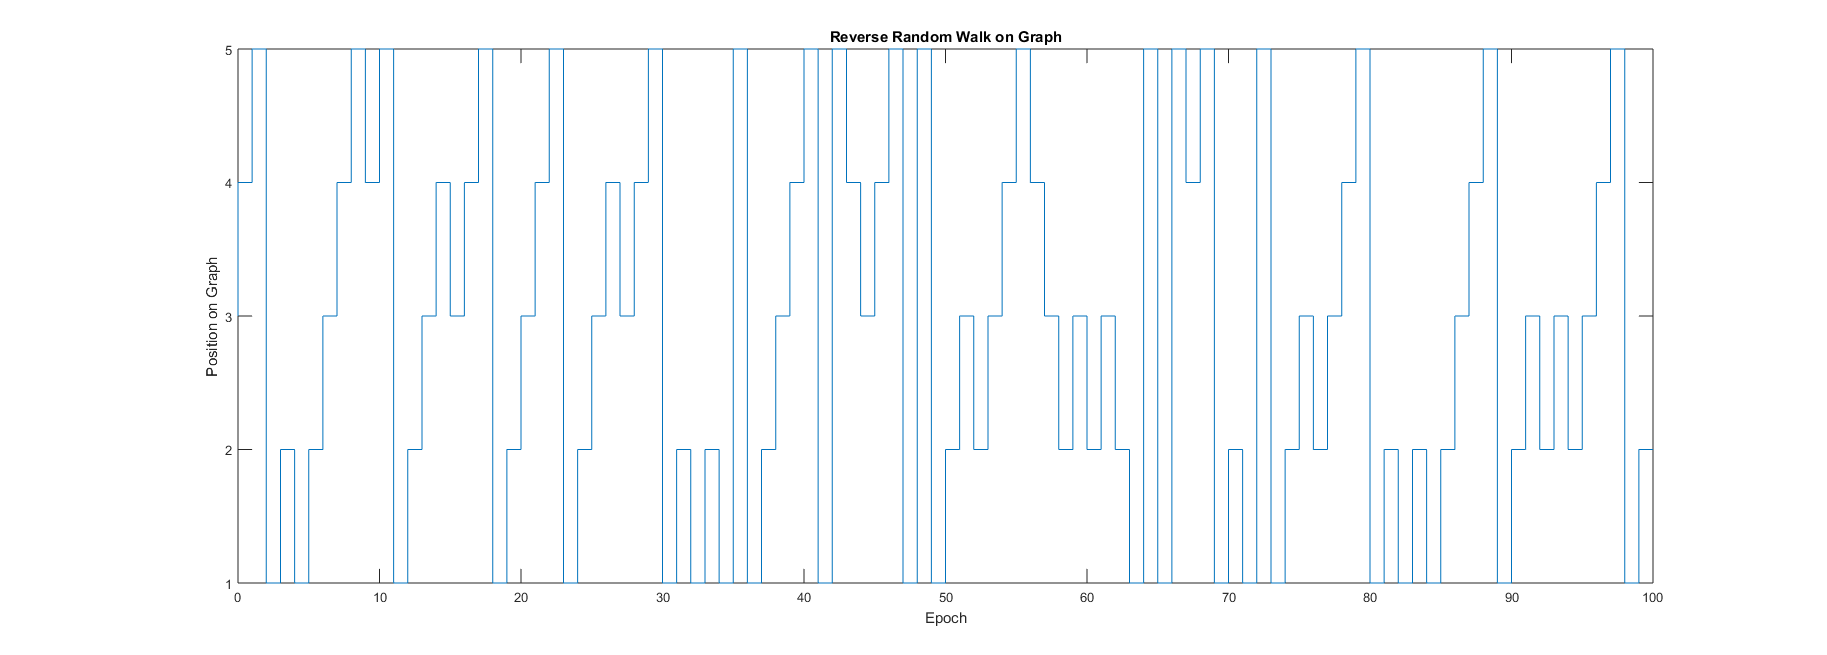
\includegraphics[scale=0.3]{ReverseRandomWalk}
\end{figure}
\begin{figure}
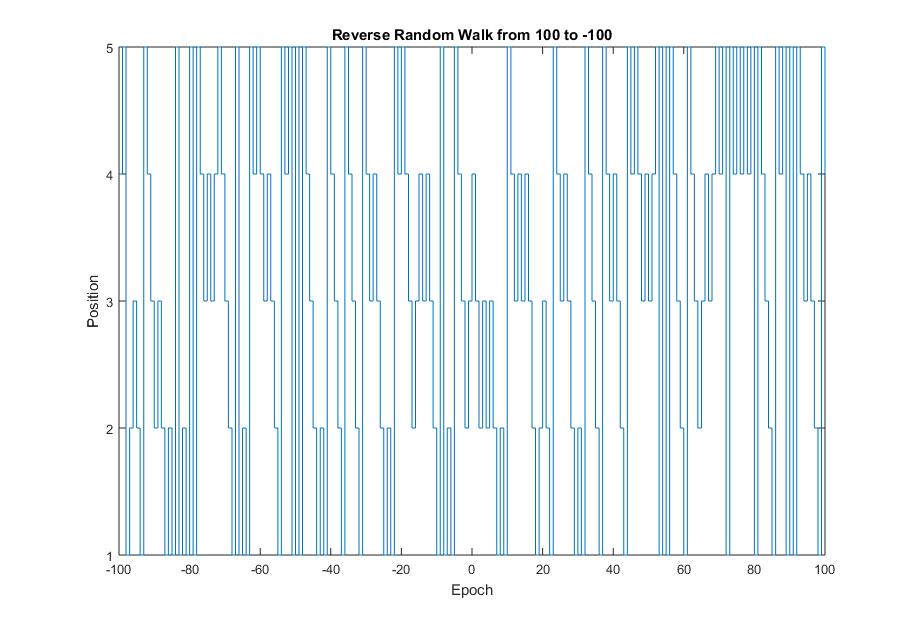
\includegraphics[scale=0.5]{ReverseRandomWalknegatives}
\end{figure}
 \end{document}




















